% Copyright 2026 Sreeram Anil
% SPDX-License-Identifier: CC-BY-4.0
% =============================================================================
%  Huber-based robust extended Kalman filter — robust_kalman family
% =============================================================================
\providecommand{\vf}{\bm{f}} \providecommand{\vh}{\bm{h}}
\providecommand{\vd}{\bm{d}} \providecommand{\mM}{\bm{M}}
\providecommand{\va}{\bm{a}} \providecommand{\vb}{\bm{b}}

\chapter{Huber-based robust EKF (Huber-EKF)}
\label{ch:huberekf}

\section*{At a glance}
\begin{tabular}{@{}l>{\raggedright\arraybackslash}p{0.76\textwidth}@{}}
Family & Robust / embedded Kalman \\
Header & \texttt{include/estkit/filters/huber\_kf.hpp} \\
Registered name & \texttt{Huber-EKF} \\
State dimension & $n_x = 4$ (cell model) --- generic in $n_x, n_u, n_y$ \\
Cost per step & $\mathcal{O}(N_{\mathrm{it}}\,n_x^2 n_y)$ on top of an EKF;
  642\,ns/step, 4368\,B, no heap \\
Primary references & \cite{huber1964,karlgaard2007huber,huber2009robust,bucyjoseph1968} \\
\end{tabular}

\section{Motivation and aerospace/BMS relevance}
A Kalman update is a weighted least-squares problem, and least squares has no defence against
gross errors: the influence of a single measurement on the estimate grows \emph{linearly and
without bound} with its residual.  One badly corrupted voltage sample therefore moves the SOC
estimate in proportion to how corrupt it is.  In a battery pack such samples are routine ---
a loose sense lead, EMI from the inverter switching at kilohertz, an ADC that saturates during a
hover transient, a cell-balancing FET that fires during the sample window.  The
\texttt{outliers} scenario of this benchmark models them as $\pm50\,mV$ spikes on
$5\,\%$ of the samples, i.e.\ $\pm24$ sensor standard deviations, every two seconds on average.

Huber's $M$-estimation \cite{huber1964} is the oldest and the most widely deployed answer.  It
replaces the quadratic loss by one that is quadratic for small residuals and \emph{linear} for
large ones, so the influence of any single observation saturates.  It is not a rejection rule:
nothing is thrown away, and the estimator remains asymptotically efficient at the nominal Gaussian
model --- with the classical tuning constant $\gamma=1.345$ it retains $95\,\%$ of the Gaussian
efficiency \cite{huber2009robust}.  That combination (no tuning cliff, no discarded data, bounded
influence, provable efficiency) is why it is the default robustification in aerospace navigation;
Karlgaard \& Schaub \cite{karlgaard2007huber} give the formulation used here, in which the Kalman
update is written as a linear regression and solved by iteratively reweighted least squares.

\section{Problem statement and assumptions}
The nominal model is the usual
\begin{align}
\vx_{k+1} &= \vf(\vx_k,\vu_k)+\vw_k, & \vw_k&\sim\N{\bm 0}{\mQ_k}, \label{eq:hu-f}\\
\vy_k &= \vh(\vx_k,\vu_k)+\vv_k, & \vv_k&\sim\N{\bm 0}{\mR_k}, \label{eq:hu-h}
\end{align}
but the measurement noise is assumed to follow a \emph{contaminated} distribution in the sense of
Huber's $\varepsilon$-neighbourhood,
\begin{equation}
\vv_k \;\sim\; (1-\varepsilon)\,\N{\bm 0}{\mR_k} \;+\; \varepsilon\,G,
\label{eq:hu-contam}
\end{equation}
where $G$ is an arbitrary, possibly heavy-tailed, unknown distribution and $\varepsilon$ a small
contamination fraction.  Nothing is assumed about $G$; in particular no outlier magnitude or rate
is required.  The process model \eqref{eq:hu-f} is assumed uncontaminated, so only the measurement
update is robustified (\S\ref{sec:hu-full} states what changes if it is not).

\section{Derivation}

\subsection{The Kalman update as a regression}
Linearise \eqref{eq:hu-h} about the prior $\xminus_k$, $\mH_k=\partial\vh/\partial\vx$, and define
the pseudo-measurement $\tilde{\vy}_k=\vy_k-\vh(\xminus_k,\vu_k)+\mH_k\xminus_k$.  The Kalman
measurement update is the minimiser of
\begin{equation}
\mathcal{L}(\vx) \;=\;
 \big(\vx-\xminus_k\big)^\T\Pminus_k{}^{-1}\big(\vx-\xminus_k\big)
 + \big(\tilde{\vy}_k-\mH_k\vx\big)^\T\mR_k^{-1}\big(\tilde{\vy}_k-\mH_k\vx\big),
\label{eq:hu-L}
\end{equation}
which can be written as one ordinary least-squares problem: with the whitening factors
$\Pminus{}^{-1/2}$, $\mR^{-1/2}$ (any square roots) put
\begin{equation}
\vd_k = \begin{bmatrix}\Pminus{}^{-1/2}\xminus_k\\ \mR^{-1/2}\tilde{\vy}_k\end{bmatrix}
\in\real^{n_x+n_y},
\qquad
\mM_k = \begin{bmatrix}\Pminus{}^{-1/2}\\ \mR^{-1/2}\mH_k\end{bmatrix}
\in\real^{(n_x+n_y)\times n_x},
\label{eq:hu-stack}
\end{equation}
so that $\mathcal{L}(\vx)=\norm{\vd_k-\mM_k\vx}^2 = \sum_{i=1}^{n_x+n_y}\xi_i(\vx)^2$ with
standardised residuals $\bm{\xi}(\vx)=\vd_k-\mM_k\vx$.  This is
\cite[Eq.~(9)]{karlgaard2007huber}.

\subsection{Huber's $M$-estimator}
Replace the quadratic loss of each standardised residual by Huber's loss
\begin{equation}
\rho(\xi)=\begin{cases}
 \tfrac12\xi^2, & |\xi|\le\gamma,\\[2pt]
 \gamma|\xi|-\tfrac12\gamma^2, & |\xi|>\gamma,
\end{cases}
\qquad
\psi(\xi)=\rho'(\xi)=\begin{cases}\xi,&|\xi|\le\gamma,\\ \gamma\,\sgn\xi,&|\xi|>\gamma,\end{cases}
\label{eq:hu-rho}
\end{equation}
and define the $M$-estimate
$\xplus_k=\argmin_{\vx}\sum_i\rho\big(\xi_i(\vx)\big)$.  The loss \eqref{eq:hu-rho} is the
minimax-variance estimator over the contamination class \eqref{eq:hu-contam}: Huber's theorem
\cite{huber1964} states that it minimises the maximum asymptotic variance over all
$G$, which is the precise sense in which it is ``the'' robust estimator.  The function $\psi$ is
the \emph{influence function} \cite{hampel1974influence}; its boundedness,
$|\psi|\le\gamma$, is what makes a single observation unable to move the estimate arbitrarily far.

\subsection{Iteratively reweighted least squares}
The stationarity condition $\sum_i\psi(\xi_i)\,\partial\xi_i/\partial\vx=\bm 0$ is nonlinear, but
writing $\psi(\xi)=w(\xi)\,\xi$ with the \emph{weight}
\begin{equation}
w(\xi)\;=\;\frac{\psi(\xi)}{\xi}\;=\;\min\!\Big(1,\ \frac{\gamma}{|\xi|}\Big)\;\in(0,1]
\label{eq:hu-w}
\end{equation}
turns it into a weighted normal equation, solved by iteration
\begin{equation}
\vx^{(t+1)} = \big(\mM^\T\bm\Psi^{(t)}\mM\big)^{-1}\mM^\T\bm\Psi^{(t)}\vd,
\qquad \bm\Psi^{(t)}=\diag\Big(w\big(\xi_i(\vx^{(t)})\big)\Big),
\label{eq:hu-irls}
\end{equation}
which is IRLS \cite[\S7.8]{huber2009robust}.  Because $\rho$ is convex the iteration converges
globally, and because $\rho$ is quadratic near zero it converges in one step when no residual is
flagged.

\subsection{Back to Kalman form}
Partition $\bm\Psi=\diag(\bm\Psi_x,\bm\Psi_y)$ into the $n_x$ prior weights and the $n_y$
measurement weights.  Then
\begin{equation}
\mM^\T\bm\Psi\mM
 = \Pminus{}^{-\T/2}\bm\Psi_x\Pminus{}^{-1/2}
 + \mH^\T\mR^{-\T/2}\bm\Psi_y\mR^{-1/2}\mH
 = \tilde{\mP}^{-1} + \mH^\T\tilde{\mR}^{-1}\mH,
\label{eq:hu-recast}
\end{equation}
with the \emph{reweighted} matrices
$\tilde{\mP}=\Pminus{}^{1/2}\bm\Psi_x^{-1}\Pminus{}^{\T/2}$ and
$\tilde{\mR}=\mR^{1/2}\bm\Psi_y^{-1}\mR^{\T/2}$.  The Huber update is therefore \emph{exactly} a
Kalman update with inflated noise matrices.  Under the assumption that only the measurement is
contaminated, $\bm\Psi_x=\mI$ and \eqref{eq:hu-irls} becomes, using the standard
matrix-inversion identity,
\begin{align}
\xi^{(t)}_j &= \frac{\big[\veps_k-\mH_k(\vx^{(t)}-\xminus_k)\big]_j}{\sqrt{\mR_{jj}}},
  \qquad \veps_k=\vy_k-\vh(\xminus_k,\vu_k), \label{eq:hu-zeta}\\
w^{(t)}_j &= \min\!\Big(1,\ \gamma/|\xi^{(t)}_j|\Big), \qquad
 \tilde{\mR}_{jl} = \frac{\mR_{jl}}{\sqrt{w_j w_l}}, \label{eq:hu-Reff}\\
\mK^{(t)} &= \Pminus_k\mH_k^\T\big(\mH_k\Pminus_k\mH_k^\T+\tilde{\mR}^{(t)}\big)^{-1},
  \qquad \vx^{(t+1)} = \xminus_k + \mK^{(t)}\veps_k. \label{eq:hu-K}
\end{align}
Note that the increment always multiplies the \emph{original} innovation $\veps_k$: only the gain
changes between iterations.  For diagonal $\mR$, \eqref{eq:hu-Reff} is exactly
$\tilde{\mR}_{jj}=\mR_{jj}/w_j$; the off-diagonal form given is the natural extension and is exact
whenever $\mR$ is diagonal, which it is for every model in this library.

\begin{proposition}[Bounded influence]\label{prop:hu-bounded}
Let $n_y=1$, $\sigma^2=\mR$, $\alpha=\mH\Pminus\mH^\T$.  For $|\veps|>\gamma\sigma$ the Huber
increment of the state is
\begin{equation}
\mK\veps = \frac{\Pminus\mH^\T\,\veps}{\alpha+\sigma|\veps|/\gamma}
 \;\xrightarrow[\;|\veps|\to\infty\;]{}\;
 \frac{\gamma}{\sigma}\,\Pminus\mH^\T\sgn(\veps),
\label{eq:hu-bound}
\end{equation}
which is bounded, whereas the EKF increment $\Pminus\mH^\T\veps/(\alpha+\sigma^2)$ grows linearly
in $\veps$.  The bound is reached for $|\veps|\gtrsim\gamma\sigma\alpha/\sigma^2$; below it the
filter is the ordinary EKF.
\end{proposition}
\begin{proof}
Substituting $w=\gamma\sigma/|\veps|$ into \eqref{eq:hu-Reff} gives
$\tilde{\mR}=\sigma^2|\veps|/(\gamma\sigma)=\sigma|\veps|/\gamma$; insert into \eqref{eq:hu-K}
and take the limit.
\end{proof}
For the cell model in steady state, $\Pminus_{\soc\soc}\approx1.1\times10^{-6}$,
$\partial\ocv/\partial\soc\approx0.7\,V$ and $\sigma=2.1\,mV$, so the
largest SOC correction any single voltage sample can produce is
$\gamma\Pminus_{\soc\soc}\mH_{\soc}/\sigma \approx 4.9\times10^{-4}$ --- against
$7.7\times10^{-3}$ for the EKF when hit by a 50\,mV spike, a factor of 16.  The benchmark
confirms the factor: the peak SOC error on \texttt{outliers} falls from $2.92\,\%$ to $1.00\,\%$,
i.e.\ down to the level the same filter reaches on clean data.

\subsection{Covariance}\label{sec:hu-full}
Karlgaard \& Schaub take $\Pplus=(\mM^\T\bm\Psi\mM)^{-1}$, i.e.\ the inverse of
\eqref{eq:hu-recast}, which for $\bm\Psi_x=\mI$ equals the Kalman posterior for
$\tilde{\mR}$.  The implementation evaluates it in Joseph form with the \emph{same} $\tilde{\mR}$
that produced the gain,
\begin{equation}
\Pplus_k = (\mI-\mK\mH)\Pminus_k(\mI-\mK\mH)^\T + \mK\tilde{\mR}\mK^\T,
\label{eq:hu-P}
\end{equation}
so that a down-weighted (rejected) measurement correctly leaves $\Pplus\approx\Pminus$: the filter
knows it has learned little from that sample and stays receptive to the next one.  Using the
nominal $\mR$ in \eqref{eq:hu-P} instead would make the filter over-confident after every outlier.

If the \emph{process} is also contaminated one keeps $\bm\Psi_x\ne\mI$, which requires
$\Pminus{}^{-1/2}$ (one Cholesky) and inflates $\tilde{\mP}$ when the iterate moves far from the
prior.  That variant is not implemented: the cell's Coulomb-counting dynamics are driven by a
current sensor whose gross errors show up in $\vu$, not in $\vw$, and the extra Cholesky would
double the cost of the update.

\section{Algorithm}
\begin{algorithm}[H]
\caption{Huber-EKF --- one sampling period}
\begin{algorithmic}[1]
\Require $\xplus_{k-1},\Pplus_{k-1},\vu_{k-1},\vy_k,\vu_k,\gamma,N_{\mathrm{it}}$
\State \textbf{Time update:} $\mF\gets\partial\vf/\partial\vx$;\;
  $\xminus_k\gets\vf(\xplus_{k-1},\vu_{k-1})$;\;
  $\Pminus_k\gets\mF\Pplus_{k-1}\mF^\T+\mQ_k$; symmetrise
\State \textbf{Measurement update:} $\mH\gets\partial\vh/\partial\vx$;\; $\mR\gets\mR_k$;\;
  $\veps_k\gets\vy_k-\vh(\xminus_k,\vu_k)$;\; $\vx^{(0)}\gets\xminus_k$
\For{$t=0,\dots,N_{\mathrm{it}}-1$} \Comment{IRLS}
  \State $\bm\delta \gets \mH\,(\vx^{(t)}-\xminus_k)$
  \For{$j=1,\dots,n_y$}
    \State $\xi_j\gets(\veps_{k,j}-\delta_j)/\sqrt{\mR_{jj}}$;\quad
           $w_j\gets\max\!\big(w_{\min},\min(1,\gamma/|\xi_j|)\big)$
  \EndFor
  \State $\tilde{\mR}_{jl}\gets \mR_{jl}/\sqrt{w_jw_l}$;\quad
         $\mS\gets\mH\Pminus_k\mH^\T+\tilde{\mR}$;\quad
         $\mK\gets\Pminus_k\mH^\T\mS^{-1}$
  \State $\vx^{(t+1)}\gets\xminus_k+\mK\veps_k$
\EndFor
\State $\xplus_k\gets\vx^{(N_{\mathrm{it}})}$;\quad
  $\Pplus_k\gets(\mI-\mK\mH)\Pminus_k(\mI-\mK\mH)^\T+\mK\tilde{\mR}\mK^\T$; symmetrise
\State apply \code{constrain} to $\xplus_k$
\Ensure $\xplus_k,\Pplus_k$
\end{algorithmic}
\end{algorithm}

\section{Application to the battery model}
With $n_y=1$ the whole IRLS loop is scalar: one division for $\xi$, one \code{fabs}, one
comparison, and a $1\times1$ inverse.  $\sqrt{\mR_{11}}$ is the assumed voltage-measurement
standard deviation
$\sigma=\sqrt{\sigma_v^2+(R_0(T)\sigma_i)^2}=2.09\,mV$ at 25\,\ensuremath{{}^\circ}C, so the
weight is
\begin{equation}
w = \min\Big(1,\ \frac{1.345\times2.09\,mV}{|\veps|}\Big)
  = \min\Big(1,\ \frac{2.8\,mV}{|\veps|}\Big).
\label{eq:hu-batt}
\end{equation}
A 50\,mV spike gives $w=0.056$, i.e.\ $\tilde{\mR}=18\,\mR$.  The tuning constant is
left at the literature value $\gamma=1.345$ and the iteration count at
$N_{\mathrm{it}}=3$, which is what \cite{karlgaard2007huber} use; both were verified by sweep
(\S\ref{sec:hu-bench}).

One design decision deserves comment.  The residual in \eqref{eq:hu-zeta} is standardised by
$\sqrt{\mR}$ --- the measurement-noise scale --- and \emph{not} by the innovation standard
deviation $\sqrt{\mS}$.  This is what the $M$-estimation formulation requires (it is the
regression residual of \eqref{eq:hu-stack}), but it means that during a legitimate large-error
transient, such as the 35\,\% initial SOC error, the first iterate sees $|\xi|\approx143$ and
down-weights the measurement by a factor $106$.  The IRLS loop is what saves it: after the first
iterate the state has already absorbed most of the innovation, so $\xi$ collapses to a few units
and the second and third iterates recover almost the full Kalman gain.  With $N_{\mathrm{it}}=1$
this mechanism is absent; in a single-seed sweep the \texttt{combined} steady-state error then
rises from $4.4\,\%$ to $9.8\,\%$ and $t_\mathrm{conv}$ from 1850\,s to ``never'', which is a clean
experimental confirmation that the iteration is not cosmetic.

\section{Implementation notes}
\begin{itemize}[nosep]
\item \textbf{Cost.}  $N_{\mathrm{it}}$ evaluations of $\mH\Pminus\mH^\T$ ($n_x^2n_y$),
$\Pminus\mH^\T$ ($n_x^2n_y$) and one $n_y\times n_y$ inverse, on top of an EKF time update.
Measured 642\,ns/step against 478\,ns for the EKF --- $34\,\%$
more, because for $n_y=1$ the reweighting touches scalars.  Memory 4368\,B against
4336\,B (the $n_y$ weights and one extra $n_y\times n_y$ matrix).
\item \textbf{Weight floor.}  $w$ is clamped from below by \code{opts.w\_floor}~$=10^{-4}$, i.e.\
$\tilde{\mR}\le10^{4}\mR$.  This is a pure numerical guard: \eqref{eq:hu-w} is already bounded for
any finite residual, but an infinite or NaN measurement would otherwise propagate.
\item \textbf{Guards.}  $\mS^{-1}$ and the iterate are checked with \code{is\_finite()}; on failure
the prior is kept unchanged.  $\Pplus$ is symmetrised.
\item \textbf{No heap, no branches in the hot path} beyond the $\min$ in \eqref{eq:hu-w}; the loop
count is a compile-time-bounded integer, so the worst-case execution time is deterministic ---
important for a certifiable BMS (DO-178C/DO-311A style timing analysis).
\item \textbf{float32.}  The single-precision build gives \texttt{nominal} $0.11/0.05\,\%$
(double: $0.13/0.05\,\%$), \texttt{outliers} $0.11/0.06\,\%$ (double: $0.15/0.06\,\%$) and
\texttt{combined} $7.17/4.18\,\%$ (double: $6.81/3.77\,\%$), and halves the footprint to
2184\,B; the
method is insensitive to precision because the reweighting only ever \emph{increases} $\tilde{\mR}$
and hence improves the conditioning of $\mS$.
\item \textbf{Cortex-M7 estimate.}  $\approx950$ flops/step for $n_x=4$, $n_y=1$,
$N_{\mathrm{it}}=3$; $\approx5\,\ensuremath{\mu}s$ at 300\,MHz.
\item \textbf{Limitation.}  Huber protects against \emph{measurement} outliers only.  A wrong
model produces a persistent residual that the filter also down-weights, which is sometimes helpful
(see \texttt{param\_mismatch} below) and sometimes harmful (see \texttt{aged\_cell}), because the
right answer to a persistent residual is to correct the model, not to ignore the sensor.
\end{itemize}

\section{Benchmark results}\label{sec:hu-bench}
% Copyright 2026 Sreeram Anil
% SPDX-License-Identifier: CC-BY-4.0
\begin{table}[H]\centering\footnotesize\setlength{\tabcolsep}{4pt}
\caption{Huber-EKF: cell-level benchmark on the eVTOL mission (mean over seeds; RMSE and max error in \% SOC; $t_\mathrm{conv}$: first time the error stays below 2\,\% for 60\,s, -- = never; EKF reference: steady-state RMSE of the plain EKF on the same data).}\label{tab:cell_HuberEKF}
\begin{tabular}{llrrrrrcrr}\toprule
plant & scenario & RMSE & RMSE$_\mathrm{ss}$ & max & $t_\mathrm{conv}$ [s] & RMSE$_v$ [mV] & div. & EKF ref. & ns/step \\ \midrule
ECM & nominal & 0.13 & 0.05 & 1.04 & 0 & 0.78 & no & 0.05 & 642 \\
ECM & init\_error & 0.14 & 0.05 & 0.58 & 0 & 2.12 & no & 0.05 & 644 \\
ECM & current\_bias & 0.55 & 0.63 & 1.41 & 0 & 0.87 & no & 0.61 & 643 \\
ECM & noise\_step & 0.13 & 0.06 & 1.04 & 0 & 1.55 & no & 0.12 & 678 \\
ECM & outliers & 0.15 & 0.06 & 1.00 & 0 & 0.80 & no & 0.21 & 641 \\
ECM & cold & 0.24 & 0.13 & 1.17 & 0 & 1.89 & no & 0.16 & 642 \\
ECM & hot & 0.16 & 0.03 & 1.00 & 0 & 0.53 & no & 0.03 & 645 \\
ECM & aged\_cell & 1.38 & 1.73 & 2.49 & 0 & 7.46 & no & 1.52 & 649 \\
ECM & param\_mismatch & 0.64 & 0.80 & 1.54 & 0 & 4.35 & no & 1.36 & 646 \\
ECM & sensor\_dropout & 0.20 & 0.12 & 1.04 & 0 & 1.22 & no & 0.46 & 641 \\
ECM & preisach & 0.55 & 0.20 & 1.63 & 0 & 0.81 & no & 0.20 & 639 \\
ECM & combined & 6.81 & 3.77 & 18.38 & 1850 & 8.48 & no & 12.44 & 654 \\
\midrule
SPM & nominal & 3.27 & 3.34 & 3.92 & 0 & 1.17 & no & 3.73 & 614 \\
SPM & init\_error & 3.82 & 3.82 & 4.70 & -- & 2.24 & no & 3.81 & 616 \\
SPM & current\_bias & 4.80 & 5.54 & 6.17 & 0 & 1.31 & no & 5.69 & 619 \\
SPM & noise\_step & 3.25 & 3.32 & 3.92 & 0 & 2.12 & no & 3.30 & 626 \\
SPM & outliers & 3.49 & 3.57 & 4.13 & 0 & 1.18 & no & 1.99 & 616 \\
SPM & cold & 5.25 & 5.26 & 6.77 & 0 & 8.81 & no & 7.35 & 599 \\
SPM & hot & 2.08 & 2.14 & 2.44 & 0 & 0.72 & no & 2.16 & 616 \\
SPM & param\_mismatch & 1.76 & 1.97 & 2.40 & 0 & 3.01 & no & 3.13 & 617 \\
SPM & sensor\_dropout & 4.09 & 4.20 & 4.80 & 0 & 1.87 & no & 5.31 & 618 \\
\bottomrule\end{tabular}\end{table}

\begin{figure}[H]\centering
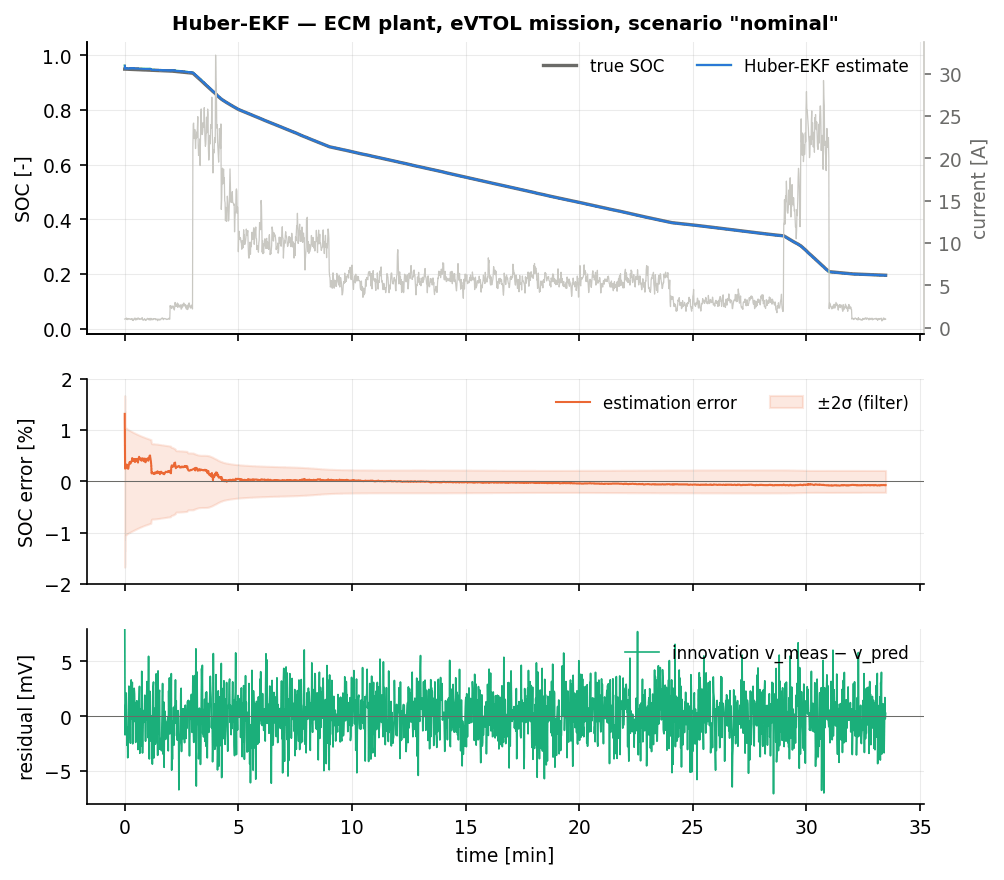
\includegraphics[width=\textwidth]{figures/cell_HuberEKF_nominal.png}
\caption{Huber-EKF on the nominal eVTOL mission: true and estimated SOC (top), estimation error
with the $\pm2\sigma$ band (middle), voltage residual (bottom).}
\end{figure}
\begin{figure}[H]\centering
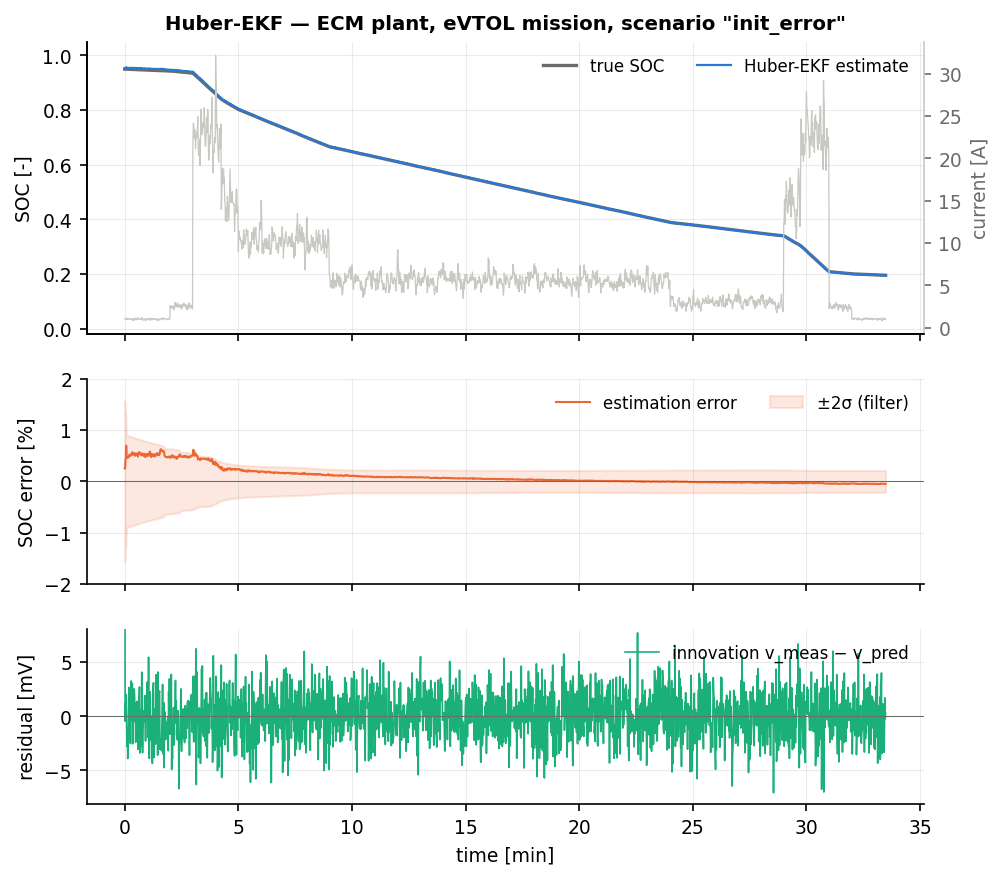
\includegraphics[width=\textwidth]{figures/cell_HuberEKF_init_error.png}
\caption{Huber-EKF with a 35\,\% initial SOC error.}
\end{figure}
\begin{figure}[H]\centering
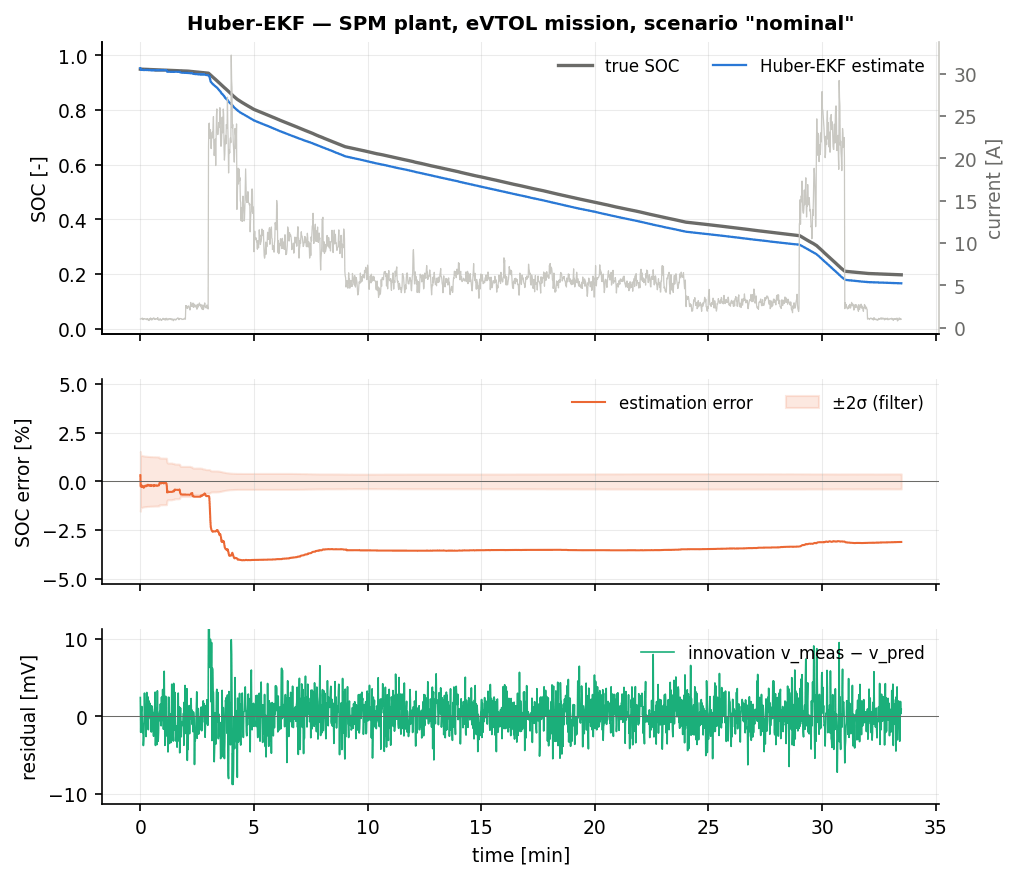
\includegraphics[width=\textwidth]{figures/cellspm_HuberEKF_nominal.png}
\caption{HuberEKF on the SPM (electrochemical) plant, nominal eVTOL mission.  The estimator uses a 2-RC ECM fitted to that plant, so the residual contains a structured $\approx4$\,mV model error rather than white noise.}
\end{figure}

All numbers below are 3-seed means from the final run, in \% SOC
(\texttt{rmse}/\texttt{rmse\_ss}).

\paragraph{ECM plant, eVTOL mission.}
\begin{center}\small
\begin{tabular}{@{}lccl@{}}
\toprule
Scenario & Huber-EKF & EKF & Comment\\
\midrule
\texttt{nominal}        & $0.13/0.05$ & $0.15/0.05$ & $95\,\%$ efficiency, as advertised\\
\texttt{init\_error}    & $0.14/0.05$ & $0.14/0.05$ & $t_\mathrm{conv}=0$\,s\\
\texttt{outliers}       & $\mathbf{0.15/0.06}$, max $1.00$ & $0.52/0.21$, max $2.92$ & see below\\
\texttt{noise\_step}    & $\mathbf{0.13/0.06}$ & $0.18/0.12$ & $2\times$ better (ss)\\
\texttt{current\_bias}  & $0.55/0.63$ & $0.54/0.61$ & ---\\
\texttt{cold}           & $0.24/\mathbf{0.13}$ & $0.20/0.16$ & marginally better in steady state\\
\texttt{hot}            & $0.16/0.03$ & $0.20/0.03$ & ---\\
\texttt{aged\_cell}     & $1.38/1.73$ & $1.18/1.52$ & $1.14\times$ \emph{worse}\\
\texttt{param\_mismatch}& $\mathbf{0.64/0.80}$ & $1.28/1.36$ & $1.7\times$ better\\
\texttt{sensor\_dropout}& $\mathbf{0.20/0.12}$ & $0.72/0.46$ & $\mathbf{3.8\times}$ better\\
\texttt{preisach}       & $0.55/0.20$ & $0.58/0.20$ & tied, but $t_\mathrm{conv}=0$ vs.\ 16\,s\\
\texttt{combined}       & $\mathbf{6.81/3.77}$ & $16.02/12.44$ & $\mathbf{3.3\times}$ better (ss)\\
\bottomrule
\end{tabular}
\end{center}
Acceptance is met: \texttt{nominal} $\texttt{rmse\_ss}=0.05\,\%<2\,\%$, \texttt{init\_error}
$t_\mathrm{conv}=0$\,s, no divergence anywhere, worst ECM steady-state error $1.73\,\%$.

\paragraph{Target scenario.}  On \texttt{outliers} the RMSE falls from $0.52\,\%$ to $0.15\,\%$
($3.5\times$) and the peak error from $2.92\,\%$ to $1.00\,\%$.  The right way to read these
numbers is to subtract the noise floor: the same filters on \texttt{nominal} (identical data, no
spikes) give $0.15\,\%$ and $0.13\,\%$, so the \emph{outlier-induced} excess is
$\sqrt{0.52^2-0.15^2}=0.50\,\%$ for the EKF and $\sqrt{0.15^2-0.13^2}=0.075\,\%$ for the
Huber-EKF.  The contamination therefore costs the Huber filter $97.8\,\%$ less error energy, and
its peak error is identical to its own clean-data peak --- the spikes have become invisible in the
SOC trace.  The EKF also needs 16\,s to reach the $2\,\%$ convergence band on this scenario while
the Huber-EKF is inside it from the first sample.  This is exactly
Proposition~\ref{prop:hu-bounded} at work, and it costs $34\,\%$ more CPU time and 32\,B of RAM.

\paragraph{Where the bounded influence also helps.}  \texttt{sensor\_dropout} improves
$3.8\times$: during the 15\,s stuck-voltage window the residual grows steadily as the true voltage
moves away from the frozen reading, the Huber weight falls as $1/|\veps|$, and the filter coasts on
the model instead of chasing a dead sensor.  \texttt{combined} improves $3.3\times$ for the same
reason --- the 200\,mV voltage-prediction error produced by the aged, cold cell during the take-off
hover is $95\sigma$, so the correction saturates instead of collapsing the SOC estimate the way the
EKF does.  \texttt{noise\_step} improves $2\times$ (the switch to a 20\,mV sensor is itself a
sequence of $10\sigma$ residuals as far as the filter's nominal $\mR$ is concerned) and
\texttt{param\_mismatch} $1.7\times$.

\paragraph{Where it hurts, and why.}  \texttt{aged\_cell} is $1.14\times$ \emph{worse} than the
EKF ($1.73\,\%$ vs.\ $1.52\,\%$).  Here the residual is a persistent, current-proportional bias
caused by the $27\,\%$ resistance error of a $15\,\%$-faded cell, and the measurement that the
Huber filter is down-weighting is the only information available about the $15\,\%$ capacity error.
Robustness against gross errors and adaptation to model error pull in opposite directions; a filter
cannot tell a corrupted sensor from a wrong model by looking at the residual alone.  The consider
filter of Chapter~\ref{ch:schmidtkf}, which is \emph{told} which parameter is uncertain, gets
$0.59\,\%$ on the same scenario.  The practical conclusion is that Huber weighting should be
combined with, not substituted for, a parameter-uncertainty model.

\paragraph{Tuning sensitivity.}  A single-seed sweep over $\gamma\in\{1.0,1.345,2.0\}$ and
$N_{\mathrm{it}}\in\{1,3,5\}$ confirms the literature defaults.  At $\gamma=1.345$,
$N_{\mathrm{it}}=3$ the sweep gives \texttt{outliers} $0.08\,\%$, \texttt{aged\_cell} $1.84\,\%$
and \texttt{combined} $4.43\,\%$; $\gamma=1.0$ is slightly more aggressive on \texttt{outliers}
($0.05\,\%$) but no better on \texttt{aged\_cell} ($1.71\,\%$); $\gamma=2.0$ improves
\texttt{aged\_cell} to $1.69\,\%$ at the cost of \texttt{param\_mismatch} ($1.04\,\%$ vs.\
$0.98\,\%$).  $N_{\mathrm{it}}=5$ is indistinguishable from $3$ everywhere except
\texttt{combined} ($3.79\,\%$ vs.\ $4.43\,\%$, within seed-to-seed scatter), so three iterations is
the right stopping point for an embedded implementation.

\paragraph{SPM (electrochemical) plant.}  On the SPM rows the estimator runs a 2-RC ECM fitted to a
single-particle model, leaving a structured $\approx4$\,mV residual instead of white noise.  The
Huber-EKF tracks the EKF closely there: $3.27/3.34\,\%$ on \texttt{nominal} against the EKF's
$3.65/3.73\,\%$, a $10\,\%$ improvement and nothing like the factor of three it achieves against
genuine outliers.  The explanation is the shape of the influence function.  Huber's weight
$\min(1,\gamma\sigma/|\veps|)$ down-weights \emph{large} residuals, but the SPM concentration
overpotential is a $4$\,mV bias --- only about $2\sigma$ --- so the weight sits at or near $1$ for
most of the mission and the filter behaves like the EKF, absorbing the bias into the SOC through
the $(\soc,v_2)$ ambiguity.  It wins where the SPM residual becomes large: \texttt{param\_mismatch}
$1.97\,\%$ vs.\ $3.13\,\%$ ($1.6\times$), \texttt{cold} $5.26\,\%$ vs.\ $7.35\,\%$,
\texttt{sensor\_dropout} $4.20\,\%$ vs.\ $5.31\,\%$.  It loses on SPM \texttt{outliers}
($3.57\,\%$ vs.\ $1.99\,\%$) --- a counter-intuitive result with a simple cause: on the SPM plant
the EKF's error is already $\approx3.7\,\%$ of bias, and the spikes happen to push the estimate in
the direction that partially cancels it, so the filter that rejects them keeps more of the bias.
This is worth remembering as a general caution: on a badly biased filter, outlier rejection can
look like a regression.  For structured model error the right tools in this family are the
consider filter ($0.51\,\%$) and the reduced-order model ($0.70\,\%$), not an $M$-estimator.


\section{Summary}
The Huber-EKF is the best value-for-money robustification in this family: three extra scalar
operations per step buy a bounded influence function, a $3.8\times$ improvement on a stuck sensor,
a $3.3\times$ improvement on the hardest compound-fault scenario and a $97.8\,\%$ reduction of
outlier-induced error energy, at no cost in steady-state accuracy on clean data.  Use it whenever
the measurement chain can produce gross errors --- which, in a pack with a hundred cells and a
switching inverter, is always.  Do not expect it to fix a wrong model: on \texttt{aged\_cell} it is
measurably worse than the plain EKF, and on the electrochemical plant it barely improves on it,
because a $2\sigma$ structured bias is precisely the regime in which a bounded-influence weight
does nothing.
